\newpage
\section{Prac 3 - I2C and PWM}
\label{sec:Prac3}
\subsection{Overview}
Before connecting to the internet for the first time, you may have noticed that the time on your Pi is a little strange. This is because the Pi doesn't have what is called an RTC (real time clock). Instead, it relies NTPD (Network Time Protocol Daemon) to fetch, set and store the date and time. However, this might be problematic as you may not always have an internet connection, and if your Pi doesn't have the correct localisation options, you may end up with the wrong time due to timezone settings. It's possible to add an RTC to the Raspberry Pi to hold the system time correctly, but for this practical we're simply going to interface with the RTC using I2C, and set the time using buttons and interrupts.

\subsubsection{Design overview}
You will be creating a modified version of a binary clock. For your convenience, an image displaying the expected operation is shown below in Figure \ref{fig:BinaryClock}.
\begin{figure}[H]
\centering
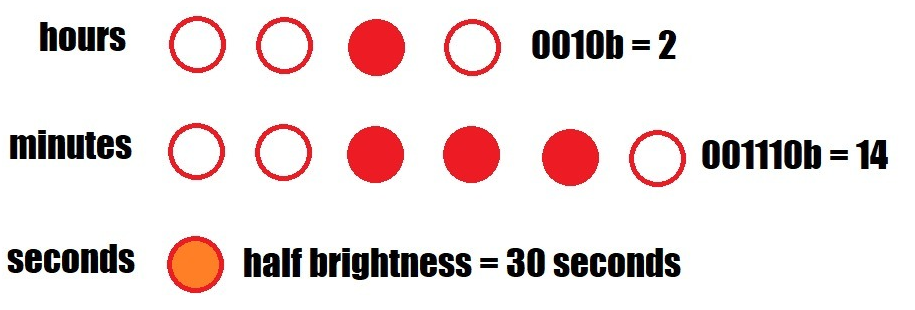
\includegraphics[width=0.6\columnwidth]{Figures/prac3clock}
\caption{A Modified Binary Clock Showing 2:14 (AM or PM)}
\label{fig:BinaryClock}
\end{figure}

Two buttons should be connected, using interrupts and \href{https://raspberrypi.stackexchange.com/questions/8544/gpio-interrupt-debounce}{debouncing}, which do the following:
\begin{enumerate}
    \item Button 1 - Fetches the hours value from the RTC, increases it by 1, and writes it back to the RTC.
    \item Button 2 - Fetches the minutes value from the RTC, increases it by 1, and writes it back to the RTC.
\end{enumerate}

You cannot use any time libraries in your script, i.e. make sure you are using the I2C communication protocol between the RTC and Pi in your script.

\subsection{Pre-prac requirements}
This section covers what you will need to know before starting the practical.
\subsubsection{Knowledge Areas}
\begin{itemize}
    \item I2C
    \item PWM
    \item Knowledge about BASH as learnt in previous pracs
    \item Read the \href{http://ww1.microchip.com/downloads/en/DeviceDoc/MCP7940M-Low-Cost\%20I2C-RTCC-with-SRAM-20002292C.pdf}{data sheet for the MCP7940M} \footnote {The Pi has onboard resistors for I2C, so you don't need to use those.}
    \item You should acquaint yourself with the Wiring Pi documentation, available \href{http://wiringpi.com/reference/}{here}.
\end{itemize}

\subsubsection{Pre-prac Submissions}
A circuit diagram for the practical. You will need to upload a schematic detailing how you are going to set up the RTC and connect it to the Raspberry Pi. It should also show how the buttons and LEDs are connected to the Pi. Software used for drawing the circuit is up to you. \footnote{You should be aware that Wiring Pi has 3 different potential modes for pin usage. Be aware of that during config and your wiring.}

\subsection{Outcomes}
You will learn about the following aspects:
\begin{itemize}
    \item I2C
    \item Real Time Clocks
    \item Wiring Pi
    \item Starting a script on boot on the Raspberry Pi
\end{itemize}

\subsection{Deliverables}
At the end of this practical, you must:
\begin{itemize}
    \item Demonstrate your working implementation to a tutor
    \item Submit your code on Vula alongside a short write-up (no more than three - 3 -  pages) detailing how you completed the practical. It is strongly recommended you do use git, but a GitHub link is not required for practical submission. See the write up format below for further guidelines. Your code and write up should be contained in a compressed folder. Your write up should be a PDF. It is not required to complete the write up using \LaTeX.
\end{itemize}

\subsection{Hardware Required}
\begin{table}[H]
\begin{tabular}{lll}
\begin{tabular}[c]{@{}l@{}}\tabitem Configured Raspberry Pi \\ \tabitem RPi Power Source\\ \tabitem Ethernet Cable\\ \tabitem A breadboard \end{tabular} & 
\begin{tabular}[c]{@{}l@{}}\tabitem 2 x push buttons\\ \tabitem 11 x LEDs (total)\\ \tabitem 11 x Resistors (total)\\ \tabitem Dupont Wires\\\end{tabular}  & 
\begin{tabular}[c]{@{}l@{}}\tabitem RTC\\ \tabitem Capacitors (kit)\\ \tabitem Crystal \\  \\\end{tabular} \\
\end{tabular}%
\end{table}


\subsection{Walkthrough}
\begin{enumerate}
    \item If you didn't in Prac 0, start by enabling I2C in raspi-config
    \item Do a git pull in the prac source folder to fetch the Prac 3 content
    \item Build the circuit you designed in the pre-prac
    \item Run \verb|$ gpio i2cdetect| to see if you can see the RTC (0x6F)
    \item Open \verb|BinClock.c| and write the code required. Some function templates are made available to give you a guide, but you may be required to write more functions as you see fit. Function definitions are placed in \verb|BinClock.h|
    \begin{itemize}
        \item Be sure to take care with regards to which pin numbering is used. You can run \verb|$ gpio readall| to check pinouts and current assignments
    \end{itemize}
    \item As a fun task, you can get the clock to run on startup using \verb|rc.local|. You can read through \href{https://www.raspberrypi.org/documentation/linux/usage/rc-local.md}{this guide}.\footnote{Admittedly, this isn't a very efficient or effective way to keep track of time. There are services that will keep track of time for us in the Pi OS, rather than us polling the RTC every second. We could even write our own code better - letting the time on the Raspberry Pi "freewheel" and having an interrupt fetch the time from the RTC every few minutes (or hours, or days or just on boot). At this point though, it becomes more sensible to simply use the hwclock service.}
\end{enumerate}

\subsection{Some Hints}
\begin{enumerate}
    \item Read the Docs. This includes the datasheet for the RTC (which you will absolutely have to do), as well as the documentation of Wiring Pi.
    \item You will need to debounce your button presses. You can use hardware debouncing, but this circuit is a bit complex, so to save space we recommend software debouncing.
    \item The source code provided to you has a lot of implementation in it already. Ensure you read and understand it before embarking out on the practical.
    \item Wiring Pi doesn't have a cleanup function like RPi.GPIO (Python). It's suggest you write your own that's caught and executed upon a keyboard interrupt. 
    \item You may notice a function called \verb|toggleTime|. This function pulls the time from the Raspberry Pi, and writes it to the LEDs. This is a nice option for "reloading" the system time to RTC.
\end{enumerate}

\subsection{Write up Format}
Your write up should consist of the following headings:
\begin{enumerate}
    \item Introduction
    \item A UML use-case diagram of the system
    \item I2C communication using Wiring Pi
    \begin{enumerate}
    \item Initialisation
    \item Send data
    \item Receive Data
    \end{enumerate}
    Include example timing diagrams in your descriptions
    \item A short paragraph on interrupts and debouncing, and why they're important in Embedded Systems (one advantage of each is enough)
    \item The circuit diagram from the pre-prac, with any changes you've made updated in the circuit diagram
\end{enumerate}